\chapter{Direct Data-Driven Control design}
\section{introduction}

In this chapter a new approach for designing controllers is going to be adopted. In general for designing controllers we have the following situations:
\begin{itemize}
    \item \textbf{Model-based controller design}: in this case, the model of the system is known and is used to design the controller in a convensional manner.
    
    \item \textbf{Data-Drive controller design}: here, the model of the system is obtained using experimental data, by means of SM identification for instance. Afterwards, the model is used in order to design the controller.
    
    \item \textbf{Direct Data-Driven controller design}: In this method, there is no need for an intermediate step of identifying the model of the system. In this appraoch, the controller is designed without knowing the model of the system and just by using the experimental input-output data.
    
\end{itemize}

In this chapter the third case is going to be discussed. The scheme we considere here is as follows: 
 \begin{figure}[H]
    \centering
    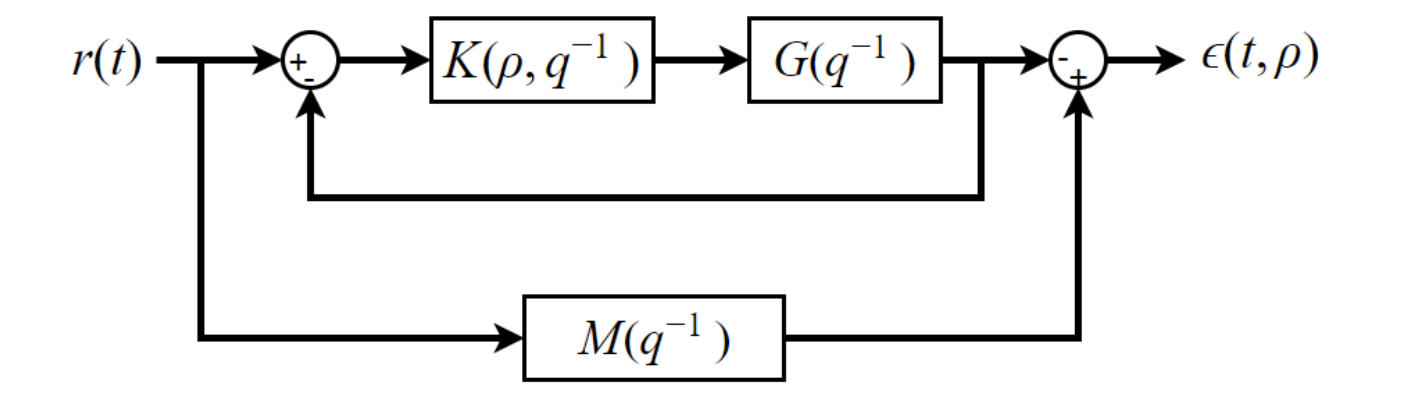
\includegraphics[width=0.75\textwidth]{dddc-scheme.png}
    \caption{Feedback control system to be designed compared with the
 reference model $M(q^{-1})$}
 \end{figure}
In this scheme, $M$ represents the \textbf{reference model}, the resultant control system, which is expected to satisfy the requirements, and $G$ is the unknown plant to be controled. 


\section{DDDC design procedure}
\subsection{Task 1: to find the controller}
The first task is to find a controller $K(\rho,\,q^{-1})$ - $K$ is an LTI discrete-time system with a transfer function depending on some parameter $\rho$ - such that the complementary sensitivity function of the controller,$T$, is close enough to the transfer function of the reference model $M$.

\[
T(q^{-1}) \approx M(q^{-1})
\]
\[
T(q^{-1}) = \frac{G(q^{-1}) K(\rho,q^{-1})}{1+G(q^{-1}) K(\rho,q^{-1})}
\]

In this equation, ideally, we expect equality for the equation above. Therefore, we are seeking to find $K$ such that:

\[
M =  \frac{G(q^{-1}) K(\rho,q^{-1})}{1+G(q^{-1}) K(\rho,q^{-1})}
\]

This problem is called, \textbf{\textit{Model matching problem}}.

\subsubsection{Result 1}
If $G(q^{-1})$ is known, the model-based matching problem has a trivial solution, which provides what we called the \textit{"ideal controller $K^{*}$"}:
\[
M + MGK = GK \Rightarrow K^{*} = \frac{M}{(1-M)G}
\]

\subsubsection{Result 2}
It can easily be shown that the ideal controller $K^{*}$
\begin{itemize}
    \item can be physically unrealisable, because the order of the denuminator of the $K^{*}$ may be large than that of the numerator. This, however, can be overcomed by suitablly adding high frequency poles.
    \item $K^{*}$ is not guaranteed to provide internal stability of the feedback control system, because $K^{*}$ is, in general, performing unstable zero-pole cancellation in $G$, which means cancelling of poles with a norm larger than 1.
\end{itemize}

\subsubsection{Result 3}
It is possible to prove that $K^{*}$ is ensuring internal stability if and only if the transfer function $M(q^{-1})$ includes all the unstable zeros of $G(q^{-1})$. \\

\subsubsection{Result 4}
Result 3 allow us to fix the second problem, to save internal stability, but what what we pay is that the modified $M(q^{-1})$ that will include het "unstable" zeros is no more a descriptoin of the describe behavior.\\

\subsubsection{Result 5}
We are assuming that $G$ is not known. Then, we can collect input-output data by performing an experiment on the plant, and we calculate the error transfer function $E$. Ideally, $E$ is zero.

\begin{factbox}
Pay attention that, here, the system $G$ must be BIBO stable so that we can perform an open-loop experiment, so the system have poles with a norm strictly smaller than 1. 
\end{factbox}

\[
E = M - \frac{G(q^{-1}) K(\rho,q^{-1})}{1+G(q^{-1}) K(\rho,q^{-1})}
\]
Here, $G$ is unknown, and $K$ is to be designed. This equation is in terms of systems and not the system output. Now, let's apply to both terms teh signal $r(t)$. By doing so, we are changing our problem to system output rather than the system. However, we have to assume that this equation can be solve for all the referecen signal.
\[
Mr =  \frac{G(q^{-1}) K(\rho,q^{-1})}{1+G(q^{-1}) K(\rho,q^{-1})}r \:\:\: \forall r(t)
\]
Here, the left side of the equation is the output of $M$ when the input $r$ is applied, and the right side of the equation is the output of the feedback control system when the same input is applied. Therefore,
\[
\mathcal{E}(t) = M.r - \frac{G(q^{-1}) K(\rho,q^{-1})}{1+G(q^{-1}) K(\rho,q^{-1})}r \:\:\: \forall r(t)
\]
where $\mathcal{E}(t)$ is the output error signal.Ideally, it should be zero for all $t$ and $r(t)$, or at any rate, it is our task.

\[
\begin{array}{c}
\mathcal{E}(t) = 0 \\
\Updownarrow \\
Mr - MKGr = KGr \\
\Updownarrow \\
(1-M)KGr = Mr\\
\Updownarrow \\
KGr = \frac{M}{1-M}
\end{array}
\]
\begin{factbox}
Pay attention that $E$ is the system error, while $\mathcal{E}(t)$ is the output error signal.
\end{factbox}

It can be seen that this equation still depends on $G$, which is not known. By replacing $Gr$ with the signal $y$.\\

Now, by simulation, considering the right-hand side of the equation, we can obtain a signal which is defined in the following manner:
\[
s(t) = \frac{M}{1-M} r(t)
\]
now, we can use the following equation for deriving the controller.
\[
K(\rho,q^{-1}) .y(t) = s(t)
\]

Finally, since through the experiment, we can obtain $\tilde{y}(k)$, so by replacing it in the equation we obtain.
\[
s(k) = K(\rho,q^{-1})[\tilde{y}(k) - \eta(k)]
\]
 \begin{figure}[H]
    \centering
    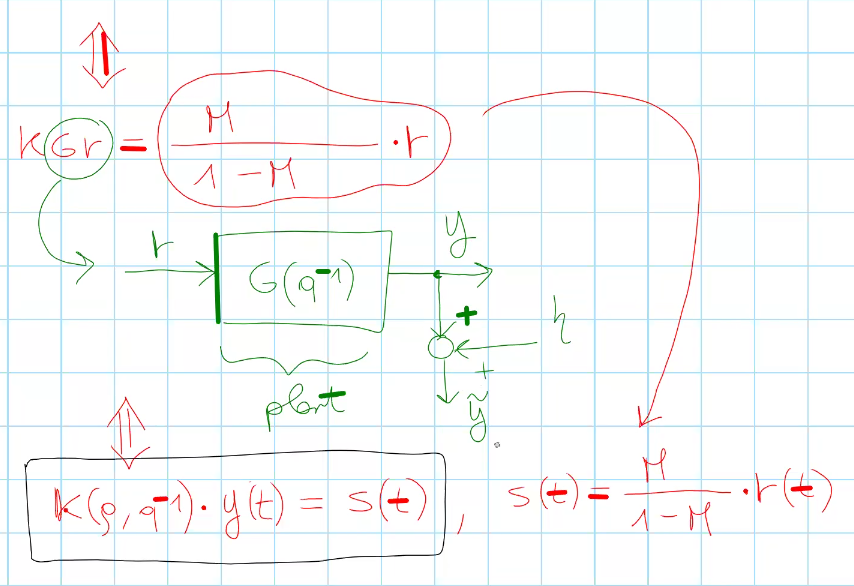
\includegraphics[width=0.65\textwidth]{dddc-prof-sketch.png}
    \caption{A graphical representation of the reasoning behind this manipulation.}
 \end{figure}
The problem of designing $K$ is infact an input-error System-identification problem under the assumption that:
\[
|\eta(k)|<\Delta\eta \:\:\: \forall k
\]
Which is a particular case of the EIV set-membership input-output problem. In order to solve ethe SM identification problem we need to select the \textbf{class of controller $C$}. e.g:
\[
C = \{\text{class of PID controllers}\}
\]
or
\[
C = \{\text{class of LTI controllers of fixed and given order}\}
\]

\textbf{How to check if $C$ is a "good" controller class?}\\
The next step in set-membership approach is to define the \textit{\textbf{Feasible Controllers Parameter set (FCPS)}}.
\[
\mathcal{D}_\rho = \{
\rho \in \mathbb{R}^{\text{length of $rho$}}: s(k) = K(\rho,q^{-1})[\tilde{y}(k) - \eta(k)],\,|\eta(k)|<\Delta\eta,\,\forall\,\,t = 1,\,2,\,\cdots,\,N
\}
\]
and then, since the description of the set is not explicit, what we do is to consider \textbf{\textit{Extended Feasible Controller Parameter Set}}, EFCPS.
\begin{example}[an example]
consider
\[
C = \{\text{class of first-order LTI controllers}\} = {K = \frac{\rho_2 + \rho_3 q^{-1}}{1 + \rho_1 q^{-1}}}
\]
for this case, FCPS becomes
\[
\mathcal{D}_\rho = \{
\rho \in \mathbb{R}^{3}: s(k) + \rho_1s(k-1) = \rho_2[\tilde{y}(k) - \eta(k)] + \rho_3[\tilde{y}(k-1) - \eta(k-1)],\,|\eta(k)|<\Delta\eta,\,\forall\,\,k = 2,\,\cdots,\,N
\]
and EFCPS becomes
\[
\mathcal{D}_{\rho,\,\eta} = \{
\rho \in \mathbb{R}^{3},\eta \in \mathbb{R}^N : s(k) + \rho_1s(k-1) = \rho_2[\tilde{y}(k) - \eta(k)] + \rho_3[\tilde{y}(k-1) - \eta(k-1)],\,|\eta(k)|<\Delta\eta,\,\forall\,\,k = 2,\,\cdots,\,N
\]
\end{example}

\textbf{Important Remark}: If $\mathcal{D}_{\rho,\,\eta}$ is empty, there is no controller in the considered class $C$ which solves the controller design problem.


\subsubsection{Result 6}
$\mathcal{D}_{\rho,\eta}$ is empty if and only if at least one of the POPs to be solved for computing the \textbf{\textit{controller parameter uncertainty intervals (CPI)}} is infeasible, which means negative exit flag in sparsepop command.
 

\subsubsection{Summerizing the controller design procedure:}
\begin{enumerate}
    \item Perform an experiment applying the reference signal $r(t)$to the plant and collect the output:
    \[
    \tilde{y}(k) = y(k) + \eta(k),\,|\eta(k)| < \Delta\eta
    \]
    
    \item Build FCPS and EFCPS
    \item compute the CPUI:
    \[
    \text{CPUI}_i = [\:\underline{\rho},\:\overline{\rho}\:]
    \]
    where
    \[
    \underline{\rho}_i = \min\limits_{\rho,\eta \in \mathcal{D}_{\rho,\,\eta}} \rho_i
    \]
    \[
    \overline{\rho}_i = \max\limits_{\rho,\eta \in \mathcal{D}_{\rho,\,\eta}} \rho_i
    \]
    \item If one of the problems is infeasible, \textbf{we have to update our controller class $C$}, which will be discussed later.
    If, on the contrary, all the POPs are feasible (positive exit flag), we obtain the CPUI for all $\rho_i$.
    \item Build the controller transfer function as:
    \[
    K(\rho,q^{-1}) = \frac{\rho_{n+1}^c + \rho_{n+1}^cq^{-2} + \cdots + \rho_{2n+1}^cq^{-n}}{1+ \rho_1^cq^{-1} + \rho_2^cq^{-2} \cdots + \rho_{n}q^{-n}}
    \]
    where $\rho_i^c$ is the Chebyshev center of the parameter $i$.
\end{enumerate}

\subsubsection{Result 7}
If $K^{*} \in C$, then $K^{*} \in \mathcal{D}_\rho$
 \begin{figure}[H]
    \centering
    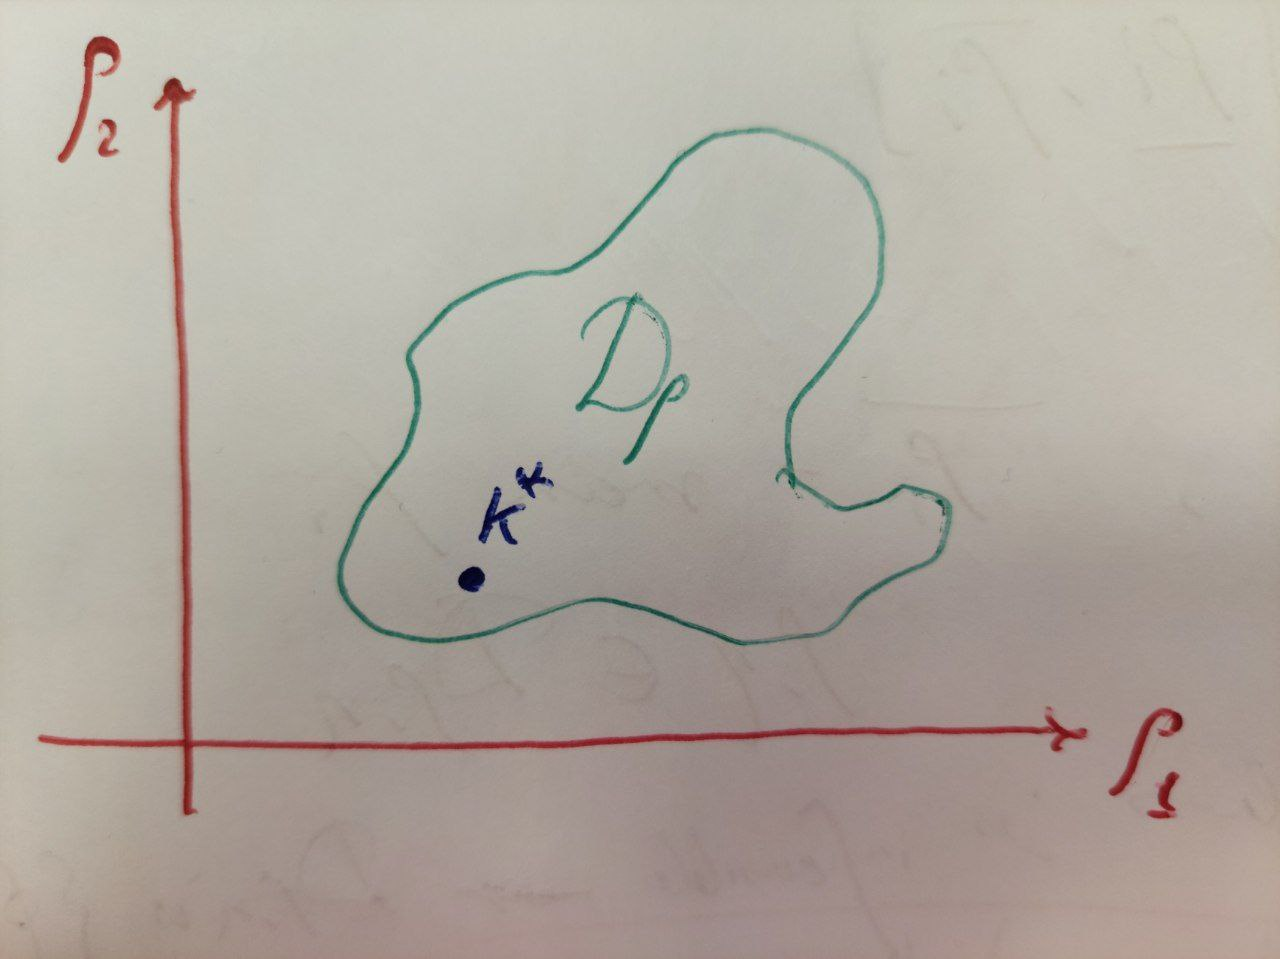
\includegraphics[width=0.65\textwidth]{d-rho.jpg}
    \caption{Feedback control system to be designed compared with the
 reference model $M(q^{-1})$}
 \end{figure}


\subsubsection{Result 8}
Since we don't know $K^{*}$, if we assume that $K^{*} \in \mathcal{D}_\rho$, the worst-case estimation of $K^{*}$ is going to be for a K on the boundary of $\mathcal{D}$ with the largest distance, so we choose $K$ to be $K(\rho^c,q^{-1})$, where
\[
\rho^c = \arg \min_{\rho \in \mathbb{R}^{\text{length of $\rho$}}} \max_{\rho' \in \mathcal{D}_\rho} \|\rho - \rho'\|_\infty
\]

considering $l_\infty$ for our cost function, $\rho^c$ becomes the Chebyshev center of the FCPS.


\subsubsection{Result 9}
It possible that the Chebyshev center in the $l_\infty$ norm is given by:
\[
\rho^c = \frac{\underline{\rho}+\overline{\rho}}{2}
\]
Since in $l_\infty$ we are considering a box around our $\mathcal{D}$ so the center of this box becomes the mean of the CPUIs.

Now, the procedure for the controller class is as follows. First, a first order model is chosen, then if it weren't feasible, the degree is increased, until we find a feasible solution.

\subsection{Considerations regarding the reference signal}
In the previous discussion, we were able to eliminate the transfer function $G(q^{-1})$ from the equation by applying the reference signal to both sides of the equation 
\[
\begin{array}{c}
\begin{cases}
E(\rho,q^{-1}) = 0\\
E(\rho,q^{-1}) = M(q^{-1}) - \frac{K(\rho,q^{-1})G(q^{-1})}{1 + K(\rho,q^{-1})G(q^{-1})}
\end{cases}
\Rightarrow M(q^{-1}) - \frac{K(\rho,q^{-1})G(q^{-1})}{1 + K(\rho,q^{-1})G(q^{-1})} = 0\\
 \Updownarrow\\
 \mathcal{E} = 0 \Leftrightarrow s(t) = K(\rho,q^{-1})\left[\tilde{y}(t)- \eta(t)\right] \:\:\:\: \forall r(t)
\end{array}
\]
And the last one should be true for all the reference signal $r$. It means that in order to try, practically, to force that equation
\[
 s(t) = K(\rho,q^{-1})\left[\tilde{y}(t)- \eta(t)\right] 
\]
is satisfied for all $r(t)$, we have to select $r(t)$ to be used in the experiment as a white noise, because \textbf{by definition as white signal is a signal having a flat spectrum at all frequencies,} which means such a signal applied to the plant is able to excite the system dynamics as well as any other signal.

\begin{factbox}[Dicussion regarding the reference signal]
If we apply a step reference signal, we are not exciting all the possible dynamics of the system, because of the spectrum of the step signal. The reason this is true is that the essential content of a step signal is the dc-gain of the signal, frequency equal to 0.\\
 \begin{figure}[H]
    \centering
    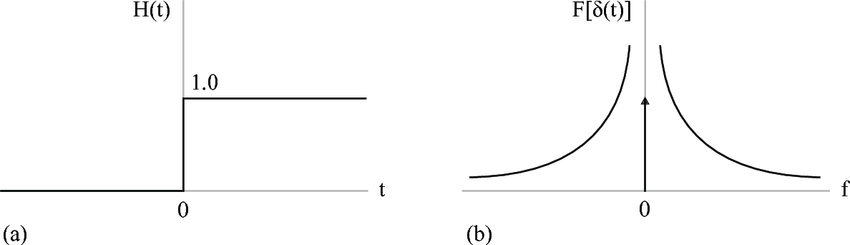
\includegraphics[width=0.65\textwidth]{step-spectrum.png}
    \caption{The frequency spectrum of step signal function}
 \end{figure}
 
 On the other hand, using a sinusoidal signal with a specific frequency stimulates the system exactly at that frequency; again you can consider the frequency response of the sinusoidal signal.\\
 
 \end{factbox}
 \begin{factbox}
 \textbf{In the procedure of designing a data-driven controller, if we pick the step reference signal, we can only say that the controller we are willing to design will be able to match the behavior of the reference system when the reference system is a step signal}. In this case, if we apply a different reference signal - for example, a sinusoidal reference signal with a high frequency - it is not guaranteed that the control system is going to match that of the reference model when that signal is applied to it.
 
In order to be able to cover all situations, in practice, we have to perform a large number of experiment considering all the signals that are of interest in our application. Afterwards, we have to collect all the data that we have obtained by different experiements. Finally, we should perform the identification using all the collected data.\\

Alternatively, if we don't know which signal is going to be used, we can use a white-noise signal to excite the plant. 

\end{factbox}


\subsection{Standard approach for selecting/designing the reference model $M_r(q^{-1})$(Not included in the exam)}
The reference model $M_r(q^{-1})$ is typically selected in order to impose a certain desired behavior to the complementary sensitivity function $T(q^{-1})$ of the feedback control system to be designed.

\begin{example}[Examples]
We can select $M_r(s)$ (continuous-time reference model) by looking at the desired step response of the feedback control system. \\

\textbf{Example 01}: to obtain a response that has the following shape,
\[
M_r(s) = \frac{1}{1+ \frac{s}{p}}, \:\:\: p > 0 
\]
which has the behavior of a stable first-order system that has a dcgain equal to 1, in order to enforce tracking the reference signal at the steady-state condition. By tuning $p$, the speed of the response can be changed.\\

\textbf{Example 02}:
A reference model that has the behavior of a second-order system.
\[
M_r(s) = \frac{\omega_n^2}{s^2 + 2 \zeta \omega_n s + \omega^2}
\]
\end{example}

\textbf{The limitation of this approach} is that by only selecting $M_r(s)$ in view of the design response of $T$, we can only impose the behavior of the feedback control system from the point of view of the reference tracking performance to one or more reference signals, but the behavior of the feedback control system as well as the attenuation of distrubrances and/or sensor noise is concerned, it is almost out of our control. \\

In fact, once we have selected $M_r(s)$ as in the previous two examples, we can obtain $M_r(q^{-1})$ by discretizing $M_r(s)$. However, the response to the disturbance $d_p$ at the output, as an example, is related to the sensitivity function of the feedback control system, which is 
\[
S(q^{-1}) = 1 - T(q^{-1})
\]
In case our desired data-driven controller is going to match exactly $M_r(q^{-1})$\\
\[
S(q^{-1}) = 1 - T(q^{-1}) = 1 - M_r(q^{-1})
\]
Nonetheless, it is not guaranteed at all that the resultant $S(q^{-1})$ is going to enjoy good attenuation property with respect to the output disturbance $d_p$ acting on the output.\\

\subsubsection{Idea (proposed approach)}
The idea is to design $M_r(q^{-1})$ by solving a \textbf{\textbf{"ficticious control design problem"}} accounting for all the quantitative performance requirements involved in the considered control problem. Here, we are refering to the following problem:\\

Assuming that our real task in a real control problem is, given a plant $G$, we want to desing a controller $K$ such that the controller have the following classes of quantitative performance requirements that accounts for:
\begin{itemize}
    \item steady-state response to polynomial reference inputs $r$
    \item steady-state response to polynomial distrubance $d_p$ 
    \item steady-state response to measurement disturbances $d_s$
    \item transient step response requirements on overshoot $\hat{s}$
    \item rise time $t_r$ and settling time $t_s$
\end{itemize}

 \subsubsection{Reference model desing in DDDC method}
 The problem addressed in the paper is to design the reference model $M$ such that the DDDC system designed on the basis of such a model meets classes of quantitative performance specifications listed above.
 
 \begin{figure}[H]
    \centering 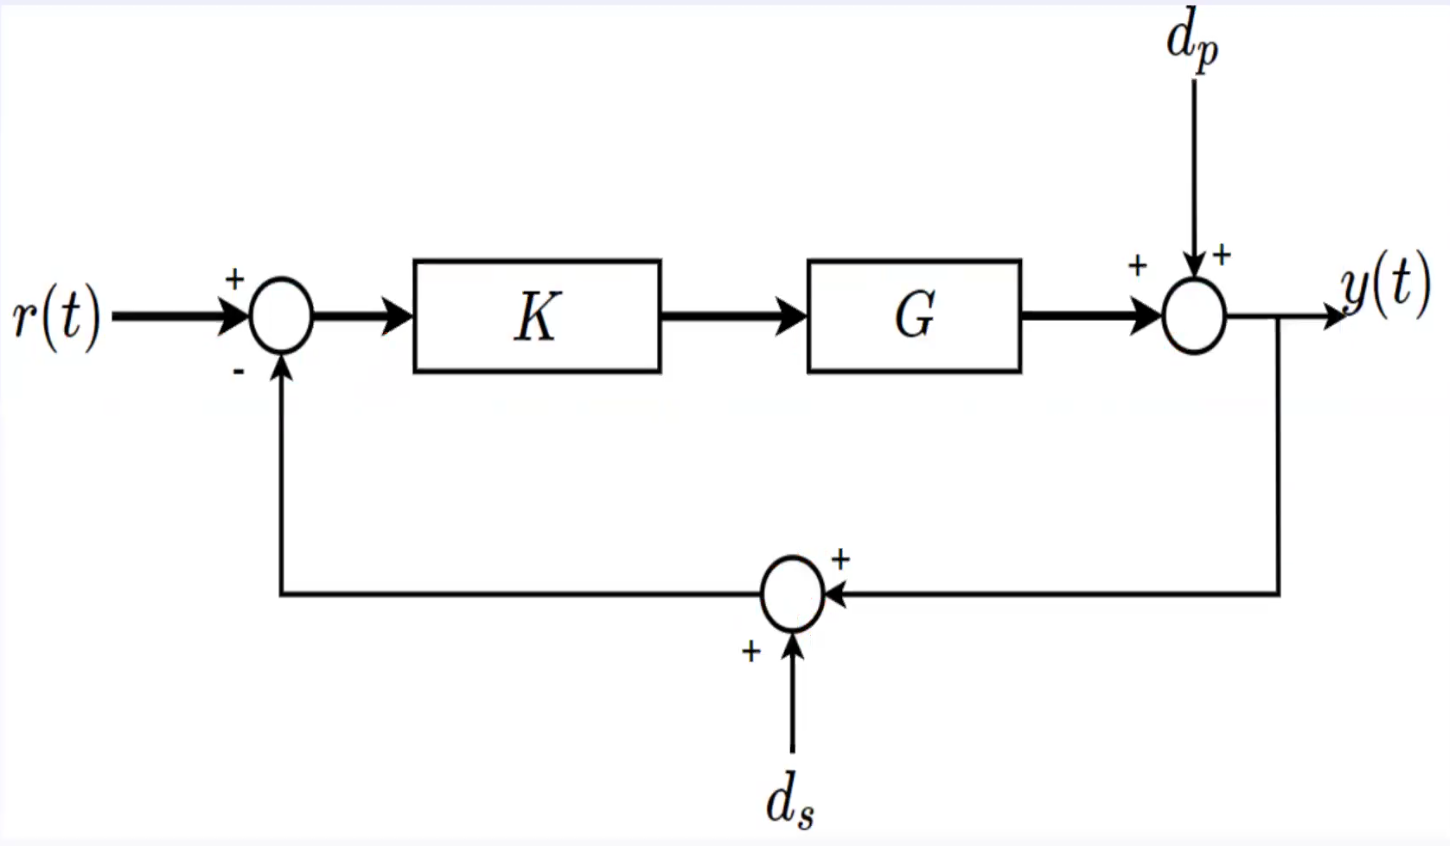
\includegraphics[width=0.65\textwidth]{fic-control-problem.png}
    \caption{The scheme of the ficticious control problem to be considered.}
 \end{figure}
 
 \subsubsection{The proposed approach}
\textbf{ I) }The main idea is that the reference model $M_r(q^{-1})$ that we are going to select will play the role of the ideal complementary sensitivity function $T(q^{-1})$ of the feedback control system. Therefore, by selecting $M_r(q^{-1})$, we can impose the reference tracking performance, but also the performance related to the attenuation of the sensor noise $d_s$.\\
 
 \textbf{II)} At the same time,  the performance related to the attenuation of the output disturbance $d_p$ depends on the shape of \\
 \[
 S(q^{-1}) = 1 - T(q^{-1}) = 1 - M_r(q^{-1})
 \]
 I and II are true since, in a feedback control system that we are considering\\
 \[
 y = T.r + Sd_p + Td_s
 \]
 If the plant $G$ is known, we can adopt any control design technique in order to design the controller. However, here, we don't know $G$. \\
  
 At this step, we don't want to obtain the controller, and, by the way, it is not possible at this stage. Now, we want to design the function $T$ and $S$ such that they satisfy the specified requirements.\\

\subsubsection{How to select the ficticious plant}
\begin{enumerate}
    \item If the true $G$\textbf{ does not have} \textit{non-minimum-phase zero} - zeros our of the unit circle:\\
    In this case, we consider a $G_{\text{ficticious}} = 1$.\\
    \begin{QandAbox}
    Because our aim at this stage is just to find what is the reference model to be obtained such that if the reference model is equal $T$, and in turn the sensitivity function $S = 1 - T$, all the requirements are satisfied. Since the behavior of the closed loop system only depends on $T$ and $S$.
     \[
 y = T.r + Sd_p + Td_s
 \]
  Then, we obtain a ficticious controller $K_{\text{ficticious}}$ that is able to control the ficticious plant satisfying the requirements. \textbf{As a result}
  \[
  T = \frac{K_{\text{ficticious}}G_{\text{ficticious}}}{1 + K_{\text{ficticious}}G_{\text{ficticious}}}
  \]
  Then, we use this $T$ for our direct-data-driven-controller problem so as to obtain the controller for the actual plant. \textbf{Since the resultant controller for the actual plant is going to result in a complementary sensitivity function $T = M_r$}, we are sure that the requirements are going to be satisfied.
    \end{QandAbox}
    \begin{example}[$H_\infty$ technique for designing the reference model (solving the ficticious control problem)]
    Condiring $H_\infty $ technique for designing the controller
     \begin{figure}[H]
    \centering 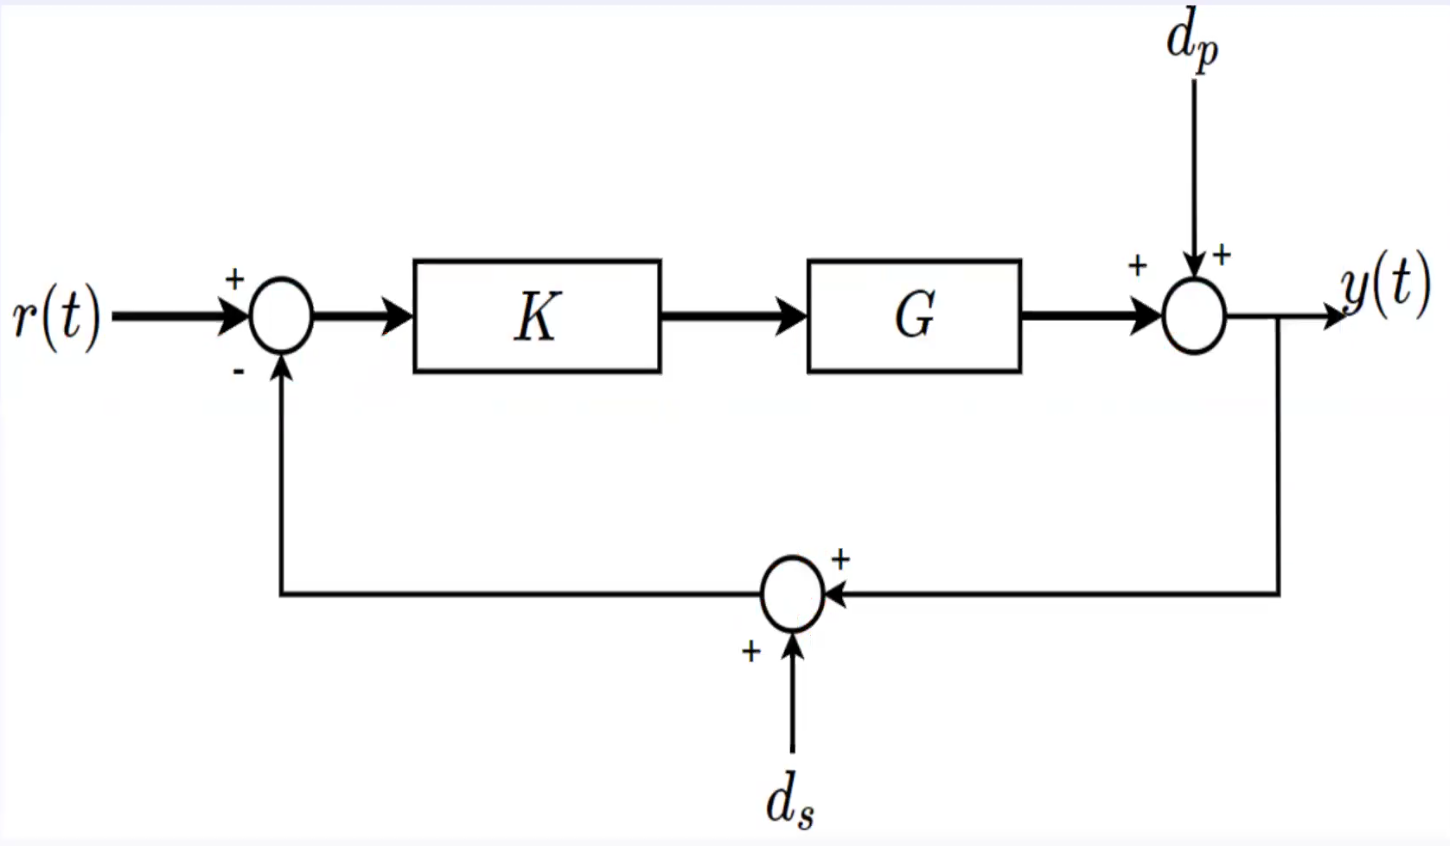
\includegraphics[width=0.6\textwidth]{fic-control-problem.png}
    \caption{The block diagram of the generalized plant used for our ficticious control problem in the $H_\infty$ context}
 \end{figure}
 As a result,
 \[
 M_r(s) = \tilde{T}(s) = \frac{\tilde{K}\tilde{G}}{1 + \tilde{K}\tilde{G}}
 \]
 where
 \[
 \tilde{K} = \arg \min\limits_{\tilde{K}(s) \in \tilde{K}(s)^{stab}} \|T_{wz}(s)\|_\infty
 \]
 and 
 \[
 T_{wz} = 
 \begin{bmatrix}
 W_T\tilde{T}\\
 W_S\tilde{S}
 \end{bmatrix}
 \]
    \end{example}
    \item The true $G$ does have zeros our of the unit circle (non-minimum-phase zeros), we have to include such zeros in the ficticious plant.\\
    If we don't consider them into the plant, while designing the controller, we obtain a $T$, it is possible that we perform an unstable cancellation with the non-minimum phase of the plant. Nonetheless,  it is a problem due to the fact that, in the context of DDDC, it is assumed that we don't know the plant.\\
    In practice, we can start by performing an experiment on $G$ by applying a step input. If the system $G$ has any non-minimum-phase zeros, the step response is going to show an undershoot. \textbf{In this case, we should do something more in order to detect the position of that zero.}
\end{enumerate}



 
 




























\section{Stability Guarantee in Set-Membership Direct Data-Driven Control}

Considering DDDC, if M and the selected controller class are ”appropriate”, a solution exists.
The DDDC procedure leads to a controller built using the central estimate $\rho^c$
\[
K^c \equiv K(q^{-1},\rho^c)
\]

It is possible that the controller that is obtained in this manner, from the SM Identification does not make the closed-loop system stable.

The fact that we have noise in the data makes the problem of determining the stability harder. If we had noise free data, we could estimate perfectly the plant, and checking the stability would have been just checking basic stability criterion for our matrix transfer function.

The noise creates a phenomenon that we obtain an infinite number of models for our plant, so we have to check the stability of all of those systems. For doing so, we have to consider the worst case inside the set.



\subsection{problem setting}

According to the DDDC frmework, stability must be established in the following conditions.
\begin{itemize}
    \item The plant $P$ is known; we assume that the order of the plant is less than or equal to a given integer $n_p$.
    \item The controller $K^c$ has been designed and is fixed.
    \item A set of input-output data $\{r_t,\tilde{y}_t)\}$ collected on the plant is available. The output samples are corrupted by noise according to:
    \[
    \tilde{y}_t = y_t + \eta_t, \hspace{0.5cm} |\eta_t|\leq \Delta_\eta, \hspace{0.5cm} t=1,\,2,\,\cdots,\,N
    \]
\end{itemize}

Uncertainty on the data makes the problem of establishing stability harder. Stability must be ensured for all allowed realizations of the noise within the specified
bound.\\

Intuition: the noise induces uncertainty on the available information.
More uncertainty means harder to achieve stability.

\subsection{$H_\infty$-norm}
$H_\infty$ in the discrete-time domain is defined as follows:
\[
\|G(z)\|_\infty  \sup\limits_{\omega \in [0,\,2\pi]} |G(e^{i\omega})|
\]
\begin{factbox}
Here, we should have an idea about the $H_\infty$, the I studied it in the modern design of control system.\\

The physical intuition about this norm is that, it gives the maximum amplification of the energy of the input that your provide to a system.
\end{factbox}

\subsection{Small-gain theorem}
Almost all the results about the robustness in control theory is based on this theorem. This theory says if two systems $S1$ and $S2$ are connected as the following figure. 

\textbf{Theorem}: Suppose subsystems $S1$ and $S2$ are stable. Then, the interconnection of these two subsystem shown in the figure is \textbf{well-posed} and \textbf{internally stable} if and only if 
\[
\|S_1S_2\|_\infty < 1
\]
It is called in this way because of the previous argument about the energy amplification interpretation of $H_\infty$ norm. 
 \begin{figure}[H]
    \centering
    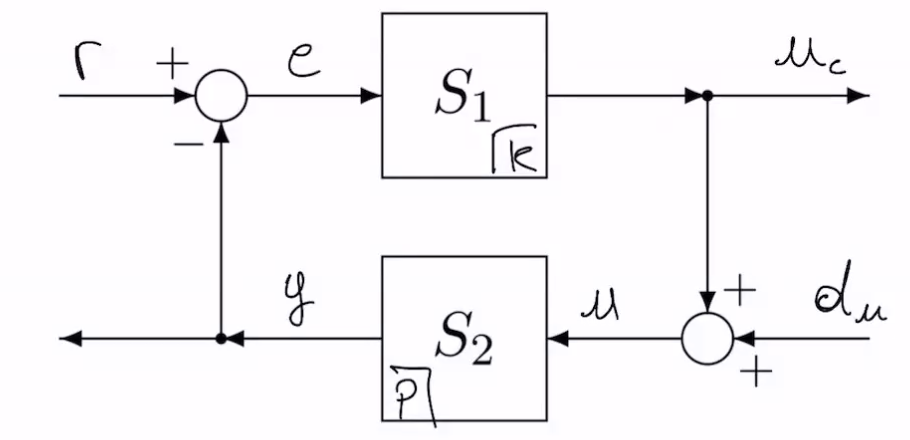
\includegraphics[width=0.4\textwidth]{interconnection-0.png}
    \caption{Inter-connection of two systems; here, S1 is considered as the controller and S2 is considered as the plant to be controlled.}
 \end{figure}


\begin{example}[Example]
Consider an unknown plant $P$. Let $P_n$ be a nominal description of the plant and $W_P$ a description of its uncertainty.\\
Assume that the model belongs to a class of multiplicative uncertainty model as follows:
\[
\{P: P = P_n (1 + W_P \Delta(z)),\,\,\|\Delta\|_\infty <1 \}
\]
Here, $P_n$ and $W_P$ are supposed to be known. \\

Now, we use the small-gain theorem. Considering the feedback control system, we consider $\Delta$ as our subsystem $S1$. 
 \begin{figure}[H]
    \centering
    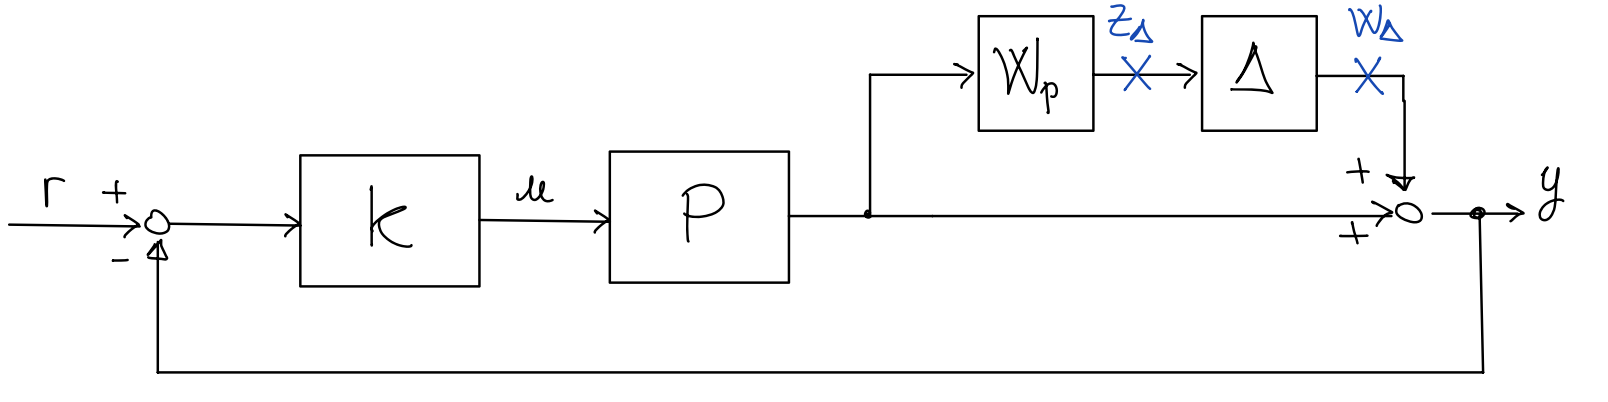
\includegraphics[width=0.75\textwidth]{small-gain-example.png}
    \caption{Block diagram of the feedback control system with uncertainty on the plant; in the discussion of indirect data drive design of controllers.}
 \end{figure}
 \[
 S1 \equiv \:\:\:\: S2 \equiv G_{w_\Delta z_\Delta} = \frac{-KP_nW_p}{1+KP_n}
 \]
 Here, $S1$ and $W_p$ is stable by assumption. Then, we should study the stability of $S2$. $S2$ is the multiplication of
 \[
 S2 = -T_n*W_p
 \]
 where
 \[
 T_n = \frac{KP_n}{1 + K P_n}
 \]
 and $T_n$ is stable if $K$ stabilizes the nominal plant.
 
 Small-gain theorem implies that:
 \[
 1 > \|S1S2\|_\infty = \|\Delta\frac{-KP_nW_P}{1 + KP_n}\|_\infty
 \]
 and adopting sum-multiplicativity property of induced norms. Induced norm is the norm defined by the worst case ratio between two norms in two different space. Since a system is an object which maps signals into signals, we can consider it as an operator between the space of signals. And if we define the norm of a signal as the energy of that signal, $H_\infty$ is the induced norm from the space of bounded energy signals.
 \[
 \|\Delta\frac{-KP_nW_P}{1 + KP_n}\|_\infty > \|\Delta\|_\infty \|\Delta\frac{KP_nW_P}{1 + KP_n}\|_\infty
 \]
 Since we know that $\|\Delta\|_\infty<1$ we obtain that 
 \[
 \|\frac{KP_nW_P}{1 + KP_n}\|_\infty < 1
 \]
 
\end{example}
\begin{example}
which means if 
\[
 \|\frac{KP_nW_P}{1 + KP_n}\|_\infty < 1
\]
the interconnection of the two systems is going to be stable two.
\end{example}


The previous example was about robust stability of a system, and, in general, any attempt to describe the uncertainty around a nominal plant inevitably leads to \textbf{indirect data-driven control}. However, in the connection of DDDC, the plant is unknown.\\

To circumvent this problem, We consider a \textbf{nominal feedback control system} with our \textbf{ideal controller}, and we consider \textbf{the uncertainty} resulting from the noisy data as a \textbf{distance between actual and ideal controller}.\\

 \begin{figure}[H]
    \centering
    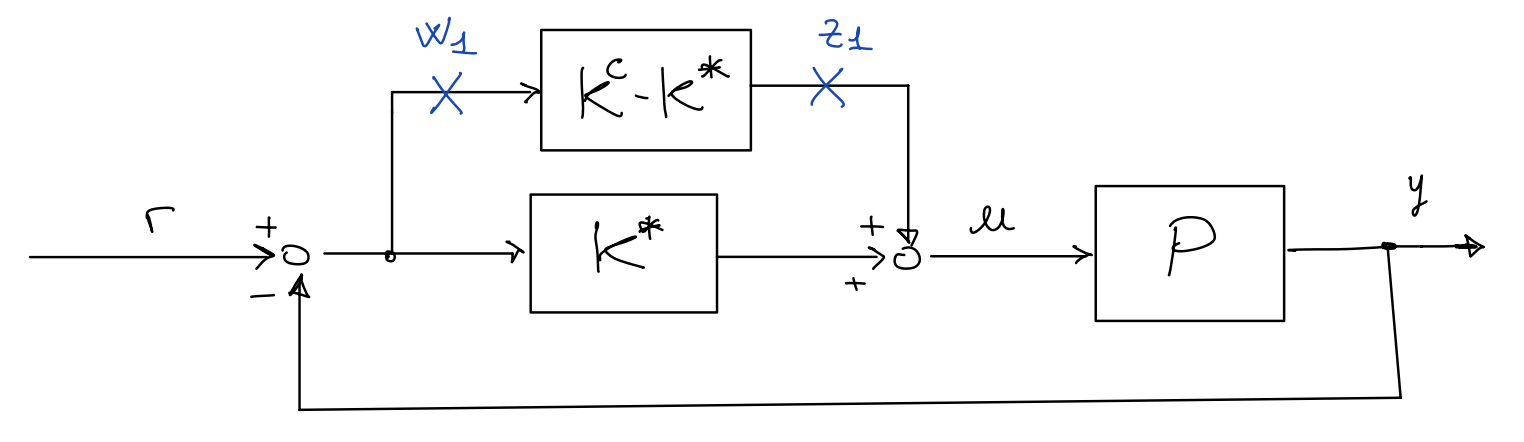
\includegraphics[width=0.75\textwidth]{small-gain-dddc.png}
    \caption{Block diagram of the feedback control system with uncertainty on the controller; this is in the context of DDDC.}
 \end{figure}

As it was discussed, $K^{*}$ is the ideal controller and the uncertainty is the distance of the ideal controller from the central controller $K^{c}$. Therefore,

\[
S1 \equiv K^{c} - K^{*} \:\:\:\: S2 \equiv \frac{-P}{1+K^{*}P} 
\]

Now consider the following theorem:\\

\textbf{Small-gain theorem in DDDC}:\\
Let
\[
\Delta(z) = M(z) - K^{c}P(z)(1-M(z))
\]
The controller $K^{c}$ stabilizes the plan $P$ if the following assumptions are satisfied:
\begin{itemize}
    \item The ideal controller $K^{*} = \frac{M}{P(1-M)}$ stabilizes the plant
    \item $\Delta(z)$ is stable
    \item $\|\Delta\|_\infty<1 $
\end{itemize}

So first, we have to show that our subsystems are stable.\\

$S2$ is the transfer function between $u$ and $y$ in the nominal system. Then, $S2$ is stable if the nominal system is stable, which means $K^{*}$ stabilizes the plant, that in turn is \textbf{our first assumption.}\\

Now, $S1$ should be stable. since $S2$ is stable then $S1$ is stable if and only if $S1S2$ is stable.\\


Let us evaluate $S1S2$
\[
S1S2 = (K^{c} - K^{*})\frac{-P}{1+K^{*}P} = \frac{K^{*}P}{1+K^{*}P} - \frac{K^{c}P}{1+K^{*}P} 
\]
It can be notices that the first term is the definition of our ideal sensitivity function and we can pull out an ideal sensitivity function from the second term.
\[
M = T^{*} = \frac{K^{*}P}{1+K^{*}P}
\]
\[
S^{*} = 1 - M = \frac{1}{1+ K^{*}P}
\]
Now, by substituting these two in our equation, the ideal controller is no longer needed to check the stability. By rewriting we obtain:
\[
M - K^{c}P(1-M)
\]
Which is what we considered $\Delta(z)$ in the description of our theorem.

$S1$ is stable if and only if $S1S2$ is stable and if and only if $\Delta$ is stable. \textbf{We consider this as our second assumption.}\\

Finally, 
\[
\|S1S2\|_\infty = \|\Delta\|_\infty < 1
\]
and this is our \textbf{assumption three}.

At this point, it is true that we eleminated $K^{*}$, but still we have the description of the plant in our theorem, which is not known in this context.


Regarding the first assumption, The ideal controller $K^{*} = \frac{M}{P(1-M)}$ stabilizes the plant \textbf{if and only if} $M$ is stable and no unstable cancellations occur, discussed in the previous section.\\
Now, we focus our attention on the second and the third assumption, which is we have to ensure that $\Delta = M - K^{c}P(1-M)$ is stable. To make sure that $Delta$ is stable we should make sure that its two terms are stable. $M$ is stable, since we want the final plant to be stable. $P$ is considered to be stable; otherwise, we would not be able to perform the experiment. $K^{c}$ is stable. Then, this condition is automatically satisfied. \\

Nevertheless, in practice, stability is not the only requirement. Most often, zero steady-error is also require, and in order to assure that, we require integrators, which make the controller unstable, and we cannot make the reasoning we just made. \\

Then we have our second sufficient condition. That is, $\Delta$ is stable if $M$ and $P$ are stable - the same reasoning as before holds - and if $K^{c}$ is \textbf{unstable only due to poles in} $z = 1$, our \textbf{loop function} $\frac{M}{1-M}$ have the same number of poles in $z = 1$.


\subsection{How to compute \(\|\Delta(z)\|_\infty\) without using the plant, and given noisy data?}

\begin{enumerate}
\item Consider one frequency at a time. Cast the problem into the SM framework. This is a set-membership \textbf{estimation} problem, \textbf{not an identification} problem, because we do not want to identify a transfer function; instead, we want to obtain a quantity related to a transfer function. We are given the following a-priori information on \(\Delta\):

\begin{itemize}
    \item Maximum order of the system: Since 
    \[
    \Delta = M - K^cP(1-M),
    \]
    we can say \(\Delta\) is a transfer function in the following form:
    \[
    \Delta(q^{-1}) = \frac{\gamma_0 + \gamma_1 q^{-1} + \cdots + \gamma_{n_\Delta}q^{-n_{\Delta}}}{1 + \delta_1 q^{-1} + \cdots + \delta_{n_\Delta}q^{-n_{\Delta}}}
    \]
    where
    \[
    n_\Delta \leq n_k + n_p + n_M.
    \]
    Here, \(n_k\) is the order of the controller \(K^c\), \(n_p\) is the order of the plant, and \(n_M\) is the order of the reference model \(M\). This relationship comes from the second term of \(\Delta\); note that \(1-M\) always has the same order as \(M\), \(n_M\).

    \item Definition and plant's data:
    \[
    \Delta(q^{-1})r_t = M(q^{-1})r_t - K^c(q^{-1})(1-M(q^{-1}))P(q^{-1})r_t 
    \]
    Now, we can substitute the following term:
    \[
    P(q^{-1})r_t = y_t = \tilde{y}_t - \eta_t
    \]
    Therefore,
    \[
    \Delta r_t = Mr_t - K^c(1-M)\tilde{y}_t + K^c (1-M)\eta_t
    \]
    here, we call name
    \[
    z_t = Mr_t - K^c(1-M)\tilde{y}_t
    \]
    and
    \[
    F(q^{-1}) = K^c (1-M)
    \]
    
    
\end{itemize}
    \item worst-case (max) norm estimation problem.
    
        \[
        \max_{\Delta,\,\eta} |\Delta(e^{i\omega})| \hspace{0.5cm} \text{s.t. } \Delta{q^{-1}}r_t = z_t + F(q^{-1})\eta_t,\,\,\,\,|\eta_t|\leq \Delta_\eta
        \]
        Pay attention that, we are not directly considering the infinity norm, and we are considering the magnitude of a values of the frequency responce for a fixed $\omega$.
        
        
        \item recast into polynomial optimization. Let $a,\,b \in \mathbb{R}$ be optimmization variables such that
        \[
        \Delta(e^{i\omega}) = a + i b
        \]
        then,
        \[
        |\Delta(e^{i\omega})| = \sqrt{a^2+b^2}\:\: \Longleftrightarrow \:\: \exists t: t=  |\Delta(e^{i\omega})|\hspace{1cm} t^2 = a^2 + b^2
        \]
        Moreover, denote:
        \[
        \begin{bmatrix}
            e^0\\
            e^{i \omega}\\
            e^{2i \omega}\\
            \vdots\\
            e^{in_\Delta \omega}
        \end{bmatrix}
        =
        \begin{bmatrix}
            \rho_0\\
            \rho_1\\
            \rho_2\\
            \vdots\\
            \rho_{n_\Delta}
        \end{bmatrix}
        +
           \begin{bmatrix}
            \sigma_0\\
            \sigma_1\\
            \sigma_2\\
            \vdots\\
            \sigma_{n_\Delta}
        \end{bmatrix}
        \]
As a function of the parameters \(\gamma,\,\delta\), we can evaluate \(\Delta(e^{i\omega})\) as:
\[
\Delta(z) = \frac{\gamma_0 z^{n_\Delta} + \gamma_1 z^{n_\Delta-1} + \cdots + \gamma_{n_\Delta-1} z + \gamma_{n_\Delta}}
{z^{n_\Delta} + \delta_1 z^{n_\Delta-1} + \cdots + \delta_{n_\Delta-1} z + \delta_{n_\Delta}}.
\]
    
    Now, we replace $z$ with $e^{i\omega}$
    \[
\Delta(e^{i\omega}) = \frac{\gamma_0 e^{i n_\Delta \omega} + \gamma_1 e^{i (n_\Delta-1) \omega} + \cdots + \gamma_{n_\Delta-1} e^{i \omega} + \gamma_{n_\Delta}}
{e^{i n_\Delta \omega} + \delta_1 e^{i (n_\Delta-1) \omega} + \cdots + \delta_{n_\Delta-1} e^{i \omega} + \delta_{n_\Delta}} = a + ib
\]
    pay attention that all the terms in $e$ are exactly known and can be considered in the vector form we denoted.

        Then $a,\,b,\,\gamma,\,\delta$ are related by:
\[
\sum_{j=0}^{n_\Delta} \gamma_j e^{i(n_\Delta-j)\omega} 
= 
(a + i b) 
\left[ 
\sum_{j=0}^{n_\Delta} \delta_j e^{i\omega (n_\Delta - j)} 
\right]
\]

here $\delta_0$ is considered to be 1 in order to make the representation more compact. Now, we replace the imaginary parts including $e$ with the cartisian representation of them.
\[
\sum_{j=0}^{n_\Delta} \gamma_j \left( \rho_j + i \sigma_j \right) 
= 
(a + i b) 
\left[ 
\sum_{j=0}^{n_\Delta} \delta_j \left( \rho_j + i \sigma_j \right) 
\right]
\]

\[
\sum_{j=0}^{n_\Delta} \gamma_j \rho_j + i \sum_{j=0}^{n_\Delta} \gamma_j \sigma_j 
= 
\sum_{j=0}^{n_\Delta} a \delta_j \rho_j + i \sum_{j=0}^{n_\Delta} a \delta_j \sigma_j 
+ i b \sum_{j=0}^{n_\Delta} \delta_j \rho_j - b \sum_{j=0}^{n_\Delta} \delta_j \sigma_j
\]

Now we get two equations, the real part on the left-hand side should be equal to the real part on the right-hand side, and the same for the imaginary part.
\[
\sum_{j=0}^{n_\Delta} \gamma_j \rho_j = \sum_{j=0}^{n_\Delta} a \delta_j \rho_j - b \sum_{j=0}^{n_\Delta} \delta_j \sigma_j
\]
For the imaginary part, we obtain:
\[
\sum_{j=0}^{n_\Delta} \gamma_j \sigma_j = + i \sum_{j=0}^{n_\Delta} a \delta_j \sigma_j 
+ i b \sum_{j=0}^{n_\Delta} \delta_j \rho_j
\]

Next, $\delta,\,\gamma$ are related to the data and the noise samples according to:

\end{enumerate}












